%Reporte sobre la actividad del producto 4
\documentclass[notitlepage,12pt]{article}

%El documento estara en español, usar paquete en español
\usepackage[spanish]{babel}
\selectlanguage{spanish}
\usepackage[utf8]{inputenc}
%Permite colores
%Permite incorporar imagenes
\usepackage{graphicx}
\usepackage{color}
%Escribir formulas matematicas
\usepackage{amsmath}
%topmatter (titulo, autor, fecha)
\title{Movimiento de proyectiles}
\author{Hugo de Jes\'us Valenzuela Chaparro}
\date{\today}

\begin{document}
\maketitle

\section{Movimiento de proyectiles o tiro parab\'olico}
El estudio de la trayectoria de un proyectil es un problema que ha sido de inter\'es por mucho tiempo. Sea 
con aplicaciones militares o en los deportes. Para estudiarse se separa en dos tipos de movimientos, un
movimiento rectil\'ineo uniforme con velocidad constante en el eje x y un movimiento rectil\'ineo uniformemente
acelerado en el eje y (con la aceleraci\'on de la gravedad). Las ecuaciones de movimiento del proyectil sin considerar
la fricción están dadas por las ecuaciones:
$x=vtcos\theta$
$y=vtsin\theta-\frac{1}{2}gt^2$
donde x y y son las variables de posición del proyectil, v es la rapidez inicial con la que se lanzó, g la aceleración 
debida a la gravedad y $\theta$ el \'angulo de lanzamiento inicial. Para determinar de forma unívoca la trayectoria de un proyectil, 
solo es necesario conocer 2 cantidades: la rapidez inicial v y el ángulo $\theta$  con el que se lanzó.

\section{C\'odigo en Fortran para el tiro parab\'olico}
A continuaci\'on se presenta un ejemplo de c\'odigo en lenguaje Fortran que ayuda a determinar la trayectoria de
un movimiento de proyectil, mandando informaci\'on de puntos a un archivo de salida, adem\'as de otros datos como 
distancia total de desplazamiento horizontal, altura m\'axima, tiempo total de vuelo. Todo esto sin considerar la
fricci\'on del aire:

\begin{verbatim}
!************************************************  
  !This program plots projectile motion of an object.  
  !The program requires user input for initial velocity   
  !and angle of the object.The algorithm uses a time   
  !step of 0.01 second i.e. it calculates object's  
  !location in the x and y plane every 0.01 second.  
  !**********By: Waleed Ishaque, 2013**************  
  program projectile_plot  
       implicit none  
       !Defining constants:  
       real, parameter :: pi = 4.0*atan(1.0) 
       real :: u, a, t, a_grados, my, mx, ft, Vx, Vy, FA  
       real, parameter :: g = 9.81  
       real:: x(150),y(150)  
          integer :: i 

       !where g is gravity, pi is "pi"   
       !u is object's initial velocity   
       !a is object's initial angle (grades)
       !t is time during the simulation   
       !x and y are arrays with 150 rows   
       !Seek user input   
       write(*,*) 'Ingresa el angulo de lanzamiento (Real)'   
       read *, a_grados   
       write(*,*) 'Ingresa la velocidad inical del proyectil en m/s (Real)'   
       read *, u   
       !Convertir angulo a radianes  
       a = (a_grados*pi)/180.0   
       !Calcular componentes de la velocidad en x (Vx) e y (Vy)
       IF (a_grados == 90.0) THEN
       Vx=0.0
       Vy=u
       ELSE IF (a_grados == 0.0) THEN
       Vx=0.0
       Vy=0.0
       ELSE
       Vx=u*cos(a)
       Vy=u*sin(a)
       END IF
        
   !Calcular el tiempo que el objeto esta en el aire, siendo el mismo
   !en las componentes x e y
   ft=(2.0*Vy)/g
 
  
   !calcular altura maxima
   my=(Vy**2)/19.62
   
   !Print results 
   print*, "Velocidad inicial:", u,"m/s"
   print*, "Angulo de lanzamiento (grados):", a_grados
   print*, "Tiempo total de vuelo:", ft, "s"
   print*, "La altura maxima es:", my,"m"
   
    
       !open .dat file and start writing on it using the algorithm   
       open(1, file='proj.dat')   
         
       
       do i=1,300 
            
            !displacement of object in x and y direction   
            t = (float(i)*0.1)   
            x(i) = Vx*t   
            y(i) = (Vy*t)-(4.905*t*t)   
            !write output in file "proj.dat" for plotting   
            write(1,*) x(i), y(i)   
            !kill the loop when the object hits the ground   
            IF (y(i)<0) exit  
       end do 
       close(1)   
       !close file 

   
  !Desplazamiento en la direccion x hasta que el objeto toca el suelo
   mx=x(i)
    print*, "El desplazamiento total en la direccion x es:", mx,"m"
  
   end program projectile_plot 
\end{verbatim}

\section{Resultados del programa corriendo}
A continuaci\'on se muestran evidencias del programa corriendo para \'angulos de 0, 30, 60 y 90
grados a una velocidad inicial de 50$\frac{m}{s}$, adem\'as de las respectivas gr\'aficas.

\subsection{$\theta=0^{\circ}$}
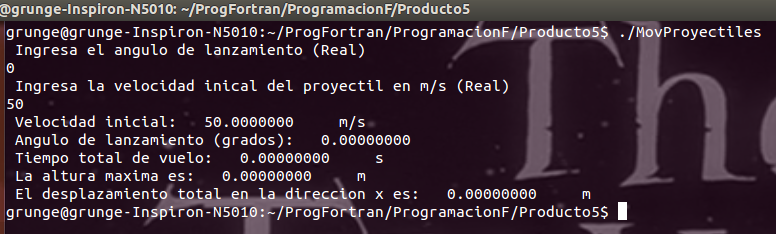
\includegraphics[scale=0.5]{teta_0}


\subsection{$\theta=90^{\circ}$}
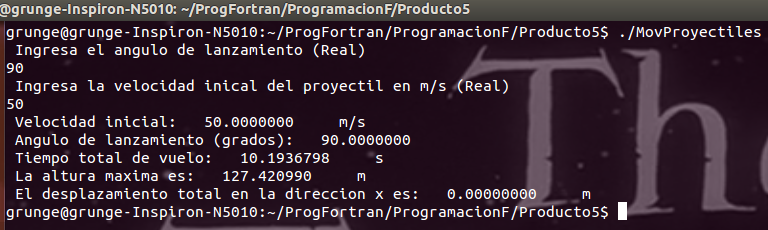
\includegraphics[scale=0.5]{teta_90}

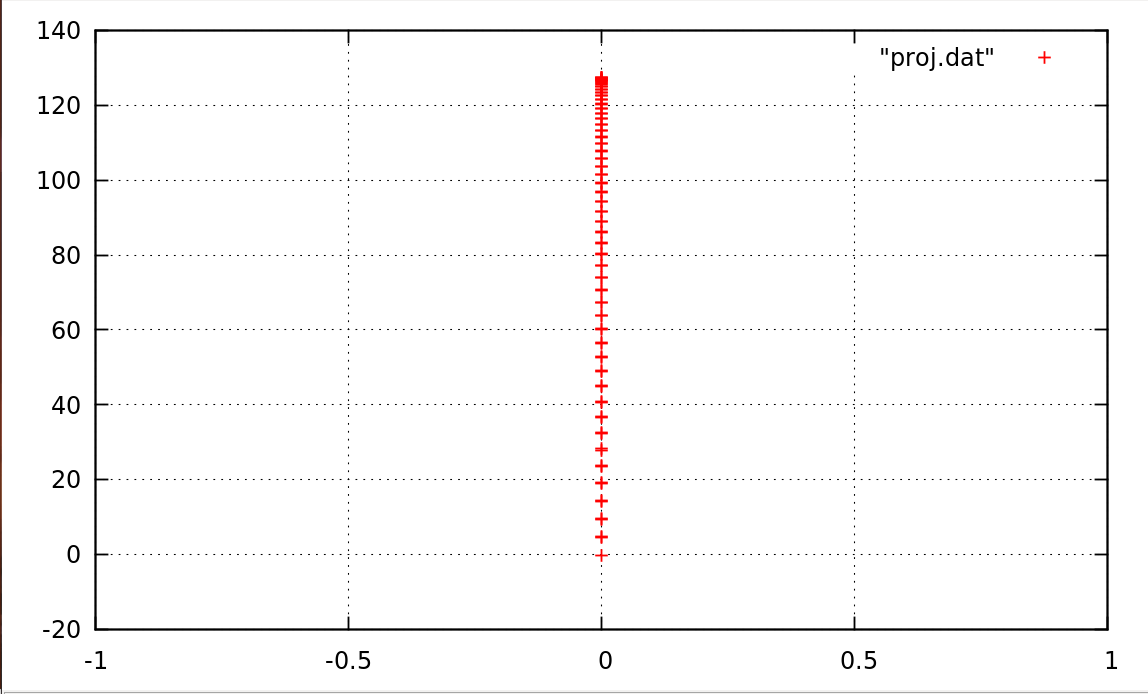
\includegraphics[scale=0.3]{grafica_teta_90}


\subsection{$\theta=30^{\circ}$}
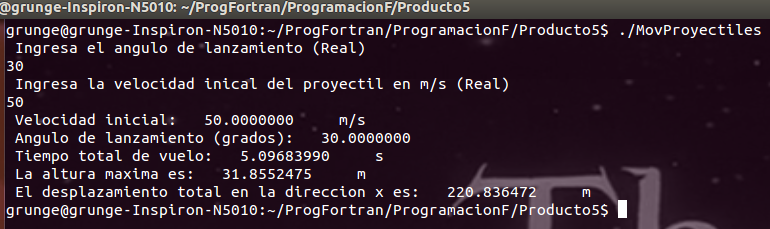
\includegraphics[scale=0.5]{teta_30}

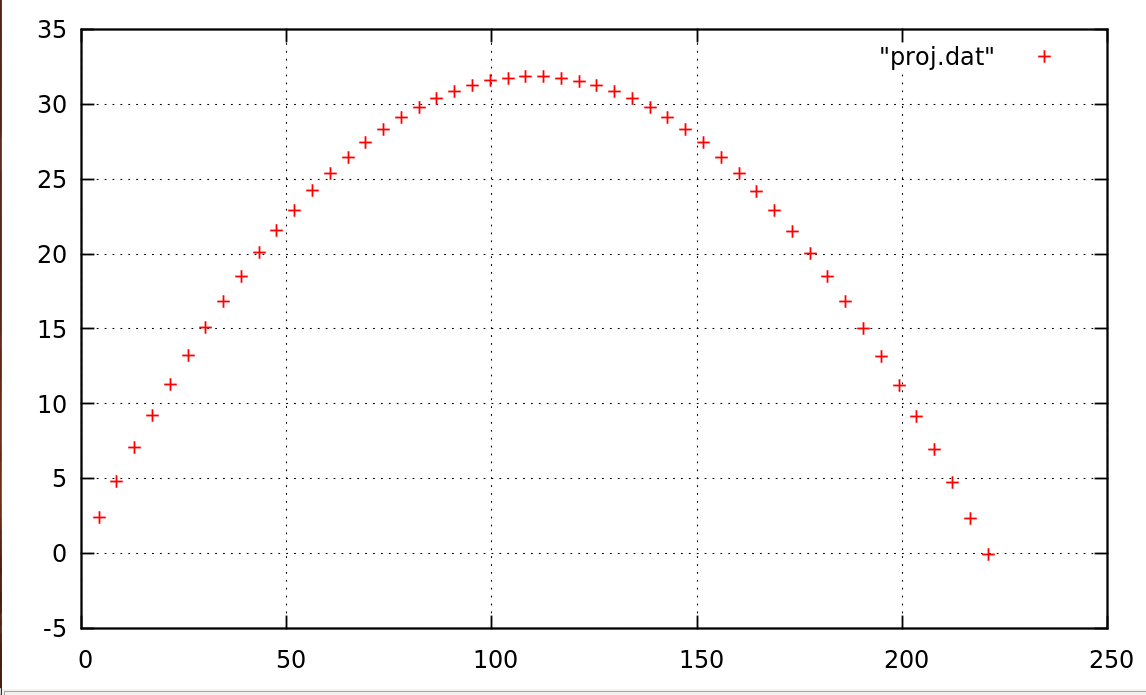
\includegraphics[scale=0.3]{grafica_teta_30}


\subsection{$\theta=60^{\circ}$}
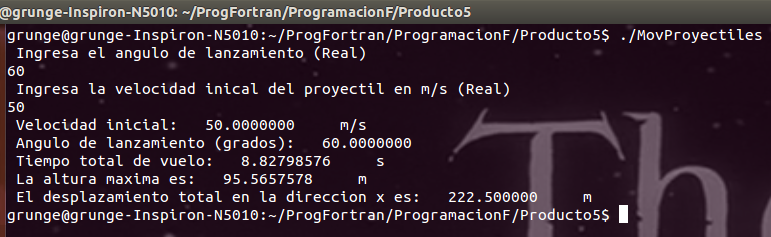
\includegraphics[scale=0.5]{teta_60}

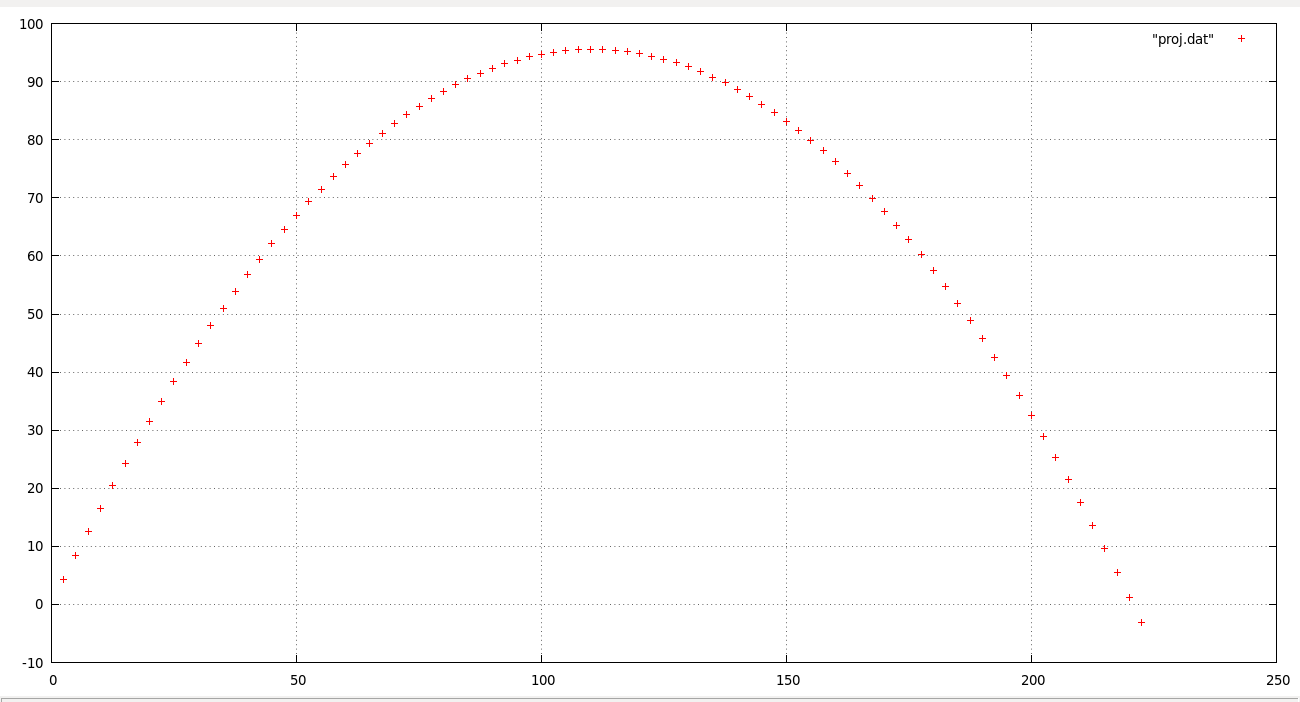
\includegraphics[scale=0.3]{grafica_teta_60}





Los resultados son consistentes, pues para un \'angulo de 0 grados no hay desplazamiento
en el eje x ni en el y, mientras que para un \'angulo de 90 grados no lo hay en el eje x
pero s\'i en el eje y (se reduce a un tiro vertical). Por otro lado, se sabe que el
desplazamiento en el eje x para \'angulos de 30 y 60 grados debe ser el mismo, mientras
que el de 60 tiene mayor altura y tarda m\'as tiempo en tocar el suelo; esto es, claro,
mientras se lanzen a la misma velocidad inicial, en el programa se nota una pequeña diferencia
en el desplazamiento x para ambos angulos, esto es debido al redondeo que hace la maquina y los
errores que se van cometiendo.













\end{document}
